% !TeX root = plantilla-trabajo.tex
\documentclass[conference,a4paper]{IEEEtran}

% Escritura mejorada de fórmulas matemáticas
\usepackage{amsmath}

% Inserción de gráficos
\usepackage{graphicx}

% Escritura de pseudocódigo
\usepackage[kw]{pseudo}

% Escritura mejorada de tablas
\usepackage{booktabs}

% Escritura mejorada de citas bibliográficas
\usepackage{cite}


% Macros traducidas
\def\contentsname{Índice general}
\def\listfigurename{Índice de figuras}
\def\listtablename{Índice de tablas}
\def\refname{Referencias}
\def\indexname{Índice alfabético}
\def\figurename{Fig.}
\def\tablename{TABLA}
\def\partname{Parte}
\def\appendixname{Apéndice}
\def\abstractname{Resumen}
% IEEE specific names
\def\IEEEkeywordsname{Palabras clave}
\def\IEEEproofname{Demostración}


\begin{document}

\title{La revolución de Othello, Bothello}

\author{
  \IEEEauthorblockN{Francisco Gago Vázquez}
  \IEEEauthorblockA{
    \textit{Dpto. Ciencias de la Computación e Inteligencia Artificial}\\
    \textit{Universidad de Sevilla}\\
    Sevilla, España\\
    fragagvaz@alum.us.es}
  \and
  \IEEEauthorblockN{Marco Antonio Herrera Luján}
  \IEEEauthorblockA{
    \textit{Dpto. Ciencias de la Computación e Inteligencia Artificial}\\
    \textit{Universidad de Sevilla}\\
    Sevilla, España\\
    marherluj@alum.us.es}
}

\maketitle


% Resumen
\begin{abstract}
  Este trabajo tiene como objetivo construir un agente dotado de Inteligencia
  artificial para el juego de mesa de ``Otelo'', el cual sea capaz de tomar
  decisiones estratégicas y estudiar su efectividad en el juego. Para ello,
  se han empleado herramientas modernas de inteligencia artificial,
  en concreto una combinación entre el algoritmo de búsqueda en árboles de
  Montecarlo (MCTS) utilizando un enfoque de Upper Confidence Bound Tree (UCT)
  combinado con la adición de aprendizaje supervisado por el uso de una Red Neuronal
  que es capaz de inferir la probabilidad de victoria dada una posición.

  Tras haber desarrollado agentes de distintos tipos, y haber estudiado su porcentaje
  de victorias respecto al de los otros modelos, hemos llegado a la conclusión de que
  ... COMPLETAR
\end{abstract}


% Palabras claves
\begin{IEEEkeywords}
  Inteligencia Artificial, Aprendizaje por Refuerzo, Aprendizaje Supervisado, 
  Red Neuronal, Montecarlo Tree Search, Othello, Reversi, Python, Pygame, otras palabras clave…
\end{IEEEkeywords}


\section{Introducción}

El siguiente trabajo se ha desarrollado en un entorno académico, con el objetivo 
de mostrar el conocimiento aprendido por los miembros del grupo durante
la asignatura ``Inteligencia Artificial'' para la evaluación del mismo, por lo que se han empleado algunas
de las técnicas y algoritmos vistos en clase para resolver el problema planteado
por el profesor. El trabajo está centrado en el universo del juego de mesa ``Otelo'',
el cual hemos modelado en el lenguaje de programación Python con ayuda de la librería
``Pygame''~\cite{b1}-~\cite{b2} apoyándonos en tutoriales de YouTube para realizar el código tanto
del juego~\cite{b3}-~\cite{b5} como del menú~\cite{b6}-~\cite{b7}. Una vez realizado el
código tanto del juego como del menú, ya podíamos jugar una persona contra otra persona, pero,
para acercarnos a nuestro objetivo de incluir agentes inteligentes, desarrollamos primero
un bot que realizara jugadas aleatorias y a su vez desarrollamos la lógica necesaria para
que al jugar contra el bot, la partida quedara registrada en un fichero csv con el texto
completamente preparado con vista a entrenar una red neuronal en el futuro.

Una vez teníamos el bot y el sistema de generación de datos, nos informamos sobre cómo
deberíamos implementar un agente~\cite{b8} para cumplir con el objetivo de atacar un problema de
búsqueda adversaria en un entorno competitivo, en concreto, en un juego determinista, de dos jugadores,
por turnos, con información perfecta y de suma cero (es decir, lo que es bueno para un jugador es un
inconveniente para su oponente).

Para crear el agente final, primero creamos un agente sin aprendizaje supervisado basándonos en el
algoritmo de búsqueda en árboles de Montecarlo (MCTS). Para construirlo, nos basamos en el pseudocódigo
descrito en la investigación de Cameron B. Browne et al. sobre los métodos de búsqueda en árbol de
Monte Carlo~\cite{b9} en el que se equilibran las fases de exploración de nodos que no tienen una fiabilidad
alta sobre su resultado con la de explotación de nodos que sí han dado buenos resultados anteriormente.

Por último, una vez terminamos el agente que implementa el algoritmo de Monte Carlo funcionando,
lo pusimos a jugar contra sí mismo para generar partidas que alimentaran a la futura red neuronal y
así poder usarla para sustituir el resultado que nos da la red dado un estado del tablero por la búsqueda
por defecto que realiza el algoritmo de Monte Carlo.

A lo largo del resto del documento, se describe el transcurso del proyecto, definiendo las técnicas
empleadas y los trabajos relacionados en los preliminares, los métodos y algoritmos utilizados en la
sección de metodología, los resultados obtenidos de la aplicación de algoritmos y métodos en la sección
de resultados, el aprendizaje obtenido de los resultados y su estudio en la sección de conclusiones y
por último las secciones de bibliografía y consultas a IA generativa.

\section{Preliminares}

Durante la realización del proyecto hemos utilizado dos técnicas principales:
el algoritmo de búsqueda en árboles de Monte Carlo (MCTS) con enfoque Upper Confidence 
Bound Tree (UCT) y el modelo de Inteligencia Artificial basado en aprendizaje supervisado 
de las redes neuronales, tal y como se ha utilizado en proyectos similares con anterioridad,
por ejemplo en juegos de mesa como el ``Go''~\cite{b10} parece que esta aproximación es 
la que mejor funciona debido a la gran complejidad que posee el juego y que por tanto hace
imposible la búsqueda de un camino óptimo como podría intentar una aproximación con el 
algoritmo MiniMax con poda alfa-beta.

\subsection{Métodos empleados}

\begin{enumerate}

  \item \textit{Upper Confidence Bound Tree}

  Nuestra aproximación para crear un agente capaz de hacer movimientos de forma estratégica
  a lo largo de la partida de Otelo, se basa en el uso del algoritmo de búsqueda en árboles
  de Monte Carlo (MCTS) con un enfoque Upper Confidence Bound Tree (UCT) como método para
  equilibrar la exploración y la explotación. La fórmula de UCT es la siguiente:
  \[
  UCT = \bar{X}_j + 2C_p \sqrt{\frac{2 \ln{n}}{n_j}} 
  \]
  donde:

  \begin{itemize}
    \item $\bar{X}_j$: es la recompensa del nodo $j$ dividida entre la cantidad de veces que 
    ha sido visitado, comprendida en el rango $[0,1]$.
    \item $C_p$: es una constante que permite regular entre el término exploratorio y el término
    explotador de la función UCT.
    \item $n$: es el número de veces que el nodo actual (nodo padre) ha sido visitado.
    \item $n_j$: es el número de veces que el hijo $j$ ha sido visitado.
  \end{itemize}

  La forma en la que $C_p$ sirve para controlar el equilibrio entre exploración y explotación
  es la siguiente:
  \begin{itemize}
    \item $\bar{X}_j$: se corresponde con el término explotador, es decir, cuanto mayor sea la
    recompensa acumulada por entrar al nodo, más probable será que se vuelva a visitar y cuantas
    más veces se haya visitado el nodo, más se favorecerá ir a otros nodos que no se hayan visitado
    tantas veces.
    \item $C_p \sqrt{\frac{2 \ln{n}}{n_j}}$: es el término exploratorio, el cual favorece que se visiten
    nodos que no han sido visitados tantas veces (por lo que no se sabe aún si darán buenas recompensas
    o no). El término disminuye cuanto mayor sea $n_j$, es decir, cuanto más se haya explorado ese nodo, mientras
    que el logaritmo del numerador asegura que la exploración decrezca lentamente a medida que se visita al
    padre. La constante, por lo tanto, sirve para controlar la importancia que se le da a la exploración
    frente a la explotación.
  \end{itemize}

  \item \textit{Monte Carlo Tree Search}
  
  El algoritmo de búsqueda en árboles de Monte Carlo ha probado ser una gran aproximación para encontrar
  la jugada óptima en juegos con información perfecta y de suma cero como el ajedrez o el Go.
  
  Este algoritmo se basa en la realización de 4 pasos diferenciados como se muestra en la Fig. 1.:

  \begin{enumerate}
  \item \textit{Selección}: Se comienza en la raíz del árbol de búsqueda y si el nodo no está expandido
  se expande. Si está expandido, devolvemos el mejor hijo según el cálculo del UCT sobre todos sus hijos.
  \item \textit{Expansión}: Teniendo un nodo no expandido, se elige una acción de las posibles acciones
  (es decir, jugadas) que se pueden realizar en ese estado del juego y se retorna el nuevo nodo. Si el nodo
  estaba expandido previamente, se llama a la función \textbf{best\_child}
  \item \textit{Simulación}: Ahora se realizan movimientos en un tablero simulado siguiendo la política
  pertinente. En un agente que implementara el MCTS sin modificaciones, se utilizaría la política por
  defecto o \textbf{default\_policy}, que en nuestro caso genera acciones de forma aleatoria hasta llegar
  a un nodo terminal. El agente que hemos implementado finalmente, sin embargo, utiliza una red neuronal
  para inferir la probabilidad de victoria o derrota dado ese nodo.
  \item \textit{Retropropagación}: Una vez obtenido el resultado de la simulación, se actualizan los valores
  tanto de recompensa como de número de visitas por nodo.
  \end{enumerate} 

  \begin{figure}
    \centering
    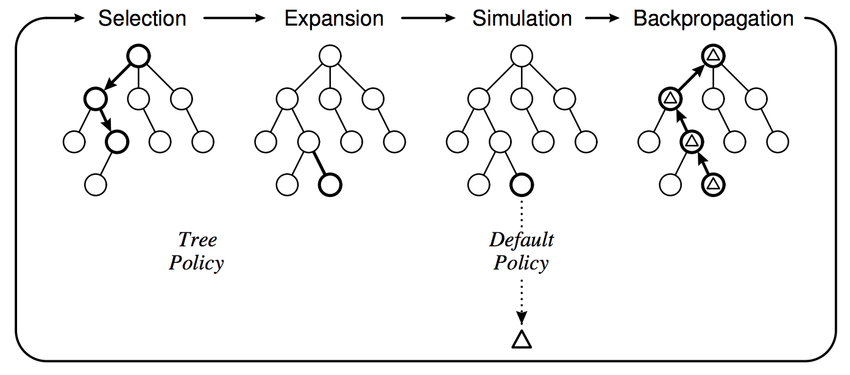
\includegraphics[width=\columnwidth]{Monte-Carlo-Tree-Search-steps-5.png}
    \caption{Esquema de funcionamiento del algoritmo MCTS~\cite{b12}.}
    \label{fig:montecarlo}
  \end{figure}

  Todos estos pasos se realizan dado un "presupuesto computacional", que normalmente es medido en tiempo
  (nuestro caso) o en número de iteraciones. Nosotros hemos obtenido buenos resultados dando 1 segundo
  para realizar los pasos anteriormente descritos.

  \item \textit{Neural Network}
  
  La red neuronal es un modelo de Inteligencia Artificial basada en aprendizaje supervisado. Para utilizarla,
  creamos un módulo encargado de generar "datos de entrenamiento" dentro de nuestro proyecto. Cada vez que
  se ejecuta una partida, se puede activar una opción que guarda cada estado $S$ de la partida con los
  siguientes datos:

  \begin{itemize}
    \item \textit{casillas}: se corresponden con cada una de las casillas del tablero. Como es de 8 filas
    y 8 columnas, van desde $a1,a2, \dots,h8$. En cada casilla se encuentran los siguientes valores:

    \begin{itemize}
      \item $0$: si en esa casilla no hay ninguna pieza.
      \item $1$: si en esa casilla hay una pieza blanca.
      \item $2$: si en esa casilla hay una pieza negra.
    \end{itemize}

    \item \textit{current\_player\_won}: se corresponde con los siguientes valores:
    
    \begin{itemize}
      \item $1$: si el jugador que estaba jugando en ese turno terminó ganando la partida.
      \item $0$: si la partida terminó en empate.
      \item $-1$: si el jugador que estaba jugando en ese turno terminó perdiendo la partida.
    \end{itemize}

  \end{itemize}

  Tras hacer que el agente de Monte Carlo jugara contra sí mismo para generar datos suficientes, creamos
  una red neuronal que, dado un nuevo estado de la partida (es decir, el estado del tablero), infiere la
  probabilidad de ganar o perder la partida en el rango $[-1,1]$.

\end{enumerate}

\subsection{Trabajo Relacionado}

El enfoque de utilizar el algoritmo de MCTS junto con una red neuronal para inferir la política no es
algo novedoso, se ha investigado en profundidad sobre el tema.

En el artículo ``\textit{Mastering the game of Go with deep neural networks and tree search}''~\cite{b10}
se explica cómo se entrenó al programa \textbf{AlphaGo} para llegar, por primera vez en el juego (el cual es
de bastante mayor complejidad que el Otelo e incluso que el ajedrez) a derrotar al campeón mundial de Go
y a todos los programas anteriormente presentados para competir en el juego de mesa.

\section{Metodología}

Esta sección se dedica a la descripción del método implementado en el trabajo.
Esta parte es la correspondiente a lo realmente desarrollado en el trabajo, y
se puede emplear pseudocódigo (nunca código), esquemas, tablas, etc.

Desarrollo del proyecto:
\begin{enumerate}
\item \textit{Preparación del proyecto:} creamos el repositorio
  en GitHub y construimos el entorno virtual de Python para el proyecto.
  Todas las dependencias necesarias se encuentran en el fichero
  \texttt{requirements.txt}.
\item \textit{Implementación de Otelo:} utilizando la librería Pygame,
  implementamos el juego de mesa Otelo, consiguiendo que dos personas
  puedan jugar entre sí.
  \begin{enumerate}
  \item \textit{Inicialización de juego:} creamos el módulo \texttt{main} 
    permitiendo abrir el juego y mostrar el tablero, y el módulo \texttt{game\_config},
    que establece constantes básicas del juego, como las dimensiones de la pantalla o 
    el tamaño del tablero.
  \item \textit{Habilitación para colocar piezas:} implementamos la clase \texttt{Board}
    y la clase \texttt{Piece}, con las funcionalidades necesarias para que los jugadores
    colocaran una ficha al hacer click en cada casilla del tablero.
  \item \textit{Aplicación de reglas de Otelo:} desarrollamos toda la lógica necesaria
    para ceñirnos a las reglas de Otelo, como la captura de piezas del oponente,
    la validación de movimientos o el cambio de turno.
  \end{enumerate} 
\item  \textit{Habilitación de bot:} programamos el juego para permitir partidas contra un
 bot controlado por el sistema, el cual escoge sus movimientos de  forma completamente aleatoria.
  \begin{enumerate}
  \item \textit{Incorporación de modos de juego:} como complemento a la creación del bot,
  añadimos la posibilidad de seleccionar entre distintos modos de juego. 
  De este modo, el usuario puede optar por jugar contra otro jugador, enfrentarse al bot, 
  o bien observar una partida controlada íntegramente por el sistema.
  \end{enumerate}

\item \textit{Creación del agente:} incorporamos un agente capaz de tomar decisiones
 estratégicas utilizando el algoritmo Monte Carlo Tree Search (MCTS).
  \begin{enumerate}
  \item \textit{Enfoque UCT:} se utilizó la variante Upper Confidence Bound Tree (UCT) 
  con el fin de equilibrar de manera efectiva la exploración y la explotación durante la búsqueda. 
  Esto permite que el algoritmo seleccione tanto las acciones con mejores resultados históricos
  como aquellas opciones menos exploradas.
  \item \textit{Elección de rol de ambos jugadores:} mejoramos la selección de modos de juego añadiendo
  la selección independiente del controlador asignado a cada jugador (humano, bot o agentes 
  con distintas políticas). De este modo, el usuario puede decidir quién controla las fichas negras 
  y quién las blancas, habilitando así todas las combinaciones posibles entre tipos de jugador.
  \end{enumerate}

\item \textit{Grabación de partidas a csv:} añadimos una funcionalidad para grabar las partidas
  jugadas en un fichero csv, de modo que posteriormente se pueda utilizar para entrenar una red 
  neuronal. Estos datos se pueden crear de manera opcional, en un archivo \texttt{.csv} que se
  genera en la carpeta \texttt{agent/training}, y toma el nombre según el tipo de partida que se
  grabe. Por tanto, si se juega una partida en la que un bot juega con las fichas negras y un agente con 
  una red neuronal \textit{NN} controla las blancas, se guardará en \texttt{agent/training/games/BOTvsAGENT\_NN.csv} 
  Posteriormente, todos estos ficheros se copiarán pasarán a otro archivo que servirá para entrenar la red.

\item \textit{Simulación de partidas:}  Para grabar datos de entrenamiento de manera automatizada,
  implementamos un sistema de generación de partidas automáticas. Con la generación de partidas,
  logramos dotar a la red neuronal de una base de datos sólida para su entrenamiento.
  
\item \textit{Red neuronal} 
  
\end{enumerate}


Las figuras se deben mencionar en el texto, como la
\figurename~\ref{fig:ejemplo}. También se pueden añadir ecuaciones, como la
ecuación~\eqref{eq:ejemplo}.

\begin{equation}
  \label{eq:ejemplo}
  a + b = \gamma
\end{equation}

Un ejemplo de pseudocódigo se puede observar en la
\figurename~\ref{pcd:mergesort}.

\begin{figure}
  \begin{pseudo}*
    \hd{\fn{mergesort}}(V) \\*
    \multicolumn{2}{l}{\textbf{Entrada}: un vector \( V \)} \\*
    \multicolumn{2}{l}{\textbf{Salida}: un vector con los elementos de \( V \)
      en orden} \\
    si \( V \) \textnormal{es unitario} entonces \\+
    devolver \( V \) \\-
    si no entonces \\+
    \( V_{1} \leftarrow \textnormal{primera mitad de } V\) \\
    \( V_{2} \leftarrow \textnormal{segunda mitad de } V\) \\
    \( V_{1} \leftarrow \pr{mergesort}(V_{1}) \) \\
    \( V_{2} \leftarrow \pr{mergesort}(V_{2}) \) \\
    devolver \fn{mezcla}(V_{1}, V_{2})
  \end{pseudo}
  
  \begin{pseudo}*
    \hd{\fn{mezcla}}(V_{1}, V_{2}) \\*
    \multicolumn{2}{l}{%
      \textbf{Entrada}: dos vectores \( V_{1} \) y \( V_{2} \) ordenados
    } \\*
    \multicolumn{2}{l}{%
      \textbf{Salida}: un vector con los elementos de \( V_{1} \) y \( V_{2} \)
      en orden
    } \\
    si \( V_{1} \) \textnormal{no tiene elementos} entonces \\+
    devolver \( V_{2} \) \\-
    si no si \( V_{2} \) \textnormal{no tiene elementos} entonces \\+
    devolver \( V_{1} \) \\-
    si no entonces \\+
    \( x_{1} \leftarrow \textnormal{primer elemento de } V_{1} \) \\
    \( x_{2} \leftarrow \textnormal{primer elemento de } V_{2} \) \\
    si \( x_{1} \leq x_{2} \) entonces \\+
    \( x \leftarrow x_{1} \) \\
    \textnormal{quitar el primer elemento de} \( V_{1} \) \\-
    si no entonces \\+
    \( x \leftarrow x_{2} \) \\
    \textnormal{quitar el primer elemento de} \( V_{2} \) \\-
    \( V \leftarrow \fn{mezcla}(V_{1}, V_{2}) \) \\
    \textnormal{añadir} \( x \)
    \textnormal{como primer elemento de} \( V \) \\
    devolver \( V \)
  \end{pseudo}
  \caption{Algoritmo de ordenación \texttt{MergeSort}}
  \label{pcd:mergesort}
\end{figure}

\section{Resultados}

Tras realizar el Bot, realizamos algunos experimentos para valorar la calidad del
agente una vez incorporada la red neuronal.
Primero comenzamos por generar partidas entre los distintos "jugadores" que teníamos,
en concreto obtuvimos los siguientes resultados:

\begin{enumerate}
\item \textit{Bot vs Bot}:
  \begin{enumerate}
    \item \textit{Configuración}\\
    Para este experimento contamos con la siguiente configuración:
    \begin{itemize}
      \item \textit{Player 1}: Bot
      \item \textit{Player 2}: Bot
    \end{itemize}
    \item \textit{Objetivo}\\
    En este experimento se quería determinar si dos jugadores que usaban siempre una
    acción aleatoria ganarían la mitad de las veces o no, por si en Otelo existiera un
    factor que favoreciera la victoria como obtener el primer turno.
    \item \textit{Resultados}\\
    Con una muestra de 250 partidas generadas, obtuvimos los siguientes resultados:
    \begin{itemize}
      \item \textit{Victorias de Player 1}: Bot
      \item \textit{Victorias de Player 2}: Bot
      \item \textit{Empates}: 
    \end{itemize}
  \end{enumerate}

\item \textit{Agente MCTS vs Bot}:
  \begin{enumerate}
    \item \textit{Configuración}\\
    Para este experimento contamos con la siguiente configuración:
    \begin{itemize}
      \item \textit{Player 1}: Agente MCTS
      \item \textit{Player 2}: Bot
      \item \textit{Valor de constante C}: $\frac{1}{\sqrt{2}}$
    \end{itemize}
    \item \textit{Objetivo}\\
    En este experimento se quería determinar si dos jugadores que usaban siempre una
    acción aleatoria ganarían la mitad de las veces o no, por si en Otelo existiera un
    factor que favoreciera la victoria como obtener el primer turno.
    \item \textit{Resultados}\\
    Con una muestra de 250 partidas generadas, obtuvimos los siguientes resultados:
    \begin{itemize}
      \item \textit{Victorias de Player 1}: Bot
      \item \textit{Victorias de Player 2}: Bot
      \item \textit{Empates}: 
    \end{itemize}
  \end{enumerate}
\end{enumerate}

Se pueden hacer uso de tablas, como el ejemplo de la tabla~\ref{tab:ejemplo}.

\begin{table}
  \caption{Ejemplo de tabla}
  \label{tab:ejemplo}
  \centering
  \begin{tabular}{ccc}
    \toprule
    A & B & C \\
    \midrule
    1 & 2 & 3 \\
    4 & 5 & 6 \\
    \bottomrule
  \end{tabular}
\end{table}


\section{Conclusiones}

Finalmente, se dedica la última sección para indicar las conclusiones obtenidas
del trabajo. Se puede dedicar un párrafo para realizar un resumen sucinto del
trabajo, con los experimentos y resultados. Seguidamente, uno o dos párrafos
con conclusiones. Se suele dedicar un párrafo final con ideas de mejora y
trabajo futuro.

\section{Uso de la IA generativa}

Durante el transcurso del proyecto, nos propusimos utilizar la Inteligencia
Artificial Generativa para cuestiones realmente necesarias, enfocando nuestras
fuentes a la hora de aprender a realizar cada una de las partes del trabajo en
fuentes de Internet (tutoriales, páginas web, documentación de librerías, etc.)
y en las lecturas recomendadas por el profesor evaluador del trabajo. Todas estas 
fuentes están incluidas dentro de la bibliografía.

En cuanto a los prompts utilizados (todos a ChatGPT), fueron los siguientes:

\begin{itemize}
\item Quiero hacer un juego en pygame, y el tablero consiste de cuadrados 
separados por lineas negras. Me preguntaba cual podria ser la mejor forma 
de recrear el tablero, si usar un asset verde del color del tablero y pintar 
de alguna forma las lineas
\item Crea una imagen de un asset para piezas de Reversi o Otelo, quiero una 
pieza blanca y una pieza negra en alta resolucion sobre un fondo verde sólido, 
para posteriormente recortarlas
\item Quiero modificar el valor de una constante que defino en otro archivo 
en mi juego de pygame en python. La importo a mi clase principal y cuando quiero 
cambiar su valor, obtengo lo siguiente: \\ \\ UnboundLocalError: cannot access 
local variable 'MODE' where it is not associated with a value
\item Estoy realizando un algoritmo basado en monte carlo tree search para 
jugar a un juego de mesa. Lo que no entiendo es cómo aprende montecarlo. Sé 
que va actualizando los nodos y guardando los valores, pero mi duda va hacia 
la implementación, ya que si lo guardo en memoria, cuando acabe la partida 
perdería toda esa información, por lo que no sé si esa información debería 
almacenarse de algún modo y, de ser así, cómo sería.
\item Estoy teniendo problemas con esta clase en la que quiero implementar el 
metodo de busqueda de montecarlo en arboles, creo que me he confundido con la 
diferencia entre nodo y estado, te adjunto la clase.
\item Teniendo en cuenta lo que me dijiste, tengo algún problema con la clase 
Board, ya que a veces se ejecuta el tablero desde el punto de vista del agente 
y otras veces se ejecuta desde el punto de vista de la persona que hace el movimiento. 
He tenido varios problemas con el constructor, ya que a veces inicializa bien 
los valores, pero cuando quiero usar la clase con montecarlo tengo problemas. 
Te adjunto la clase.
\item Te voy a enviar una red neuronal. La idea es que un agente la llame para 
que haga predicciones, pero no se si esta es la forma correcta de hacerlo 
(organización de código, tener cuidado en que si hay dos agentes no se sobreescriban 
los datos de ambos objetos, etc)
\item Puedes explicarme en mayor detalle qué es el upper bound confidence tree
en el contexto de Monte Carlo Tree Search algorithm?
\end{itemize}

\begin{thebibliography}{00}
\bibitem{b1} Documentación de Pygame. \\ Disponible en: https://www.pygame.org/docs/
\bibitem{b2} Tutorial sobre Pygame. \\ Disponible en: https://pygame.readthedocs.io/en/latest/index.html
\bibitem{b3} Tutorial para hacer las damas en Pygame (Parte 1). Disponible en:\\ https://www.youtube.com/watch?v=vnd3RfeG3NM\&list=PLzMcBGfZo4-lkJr3sqpikNyVzbNZLRiT3
\bibitem{b4} Tutorial para hacer las damas en Pygame (Parte 2). Disponible en:\\ https://www.youtube.com/watch?v=LSYj8GZMjWY\&list=PLzMcBGfZo4-lkJr3sqpikNyVzbNZLRiT3\&index=2
\bibitem{b5} Tutorial para hacer las damas en Pygame (Parte 3). Disponible en:\\ https://www.youtube.com/watch?v=\_kOXGzkbnps\&list=PLzMcBGfZo4-lkJr3sqpikNyVzbNZLRiT3\&index=3
\bibitem{b6} Tutorial para hacer el menú en Pygame. Disponible en:\\ https://www.youtube.com/watch?v=GMBqjxcKogA
\bibitem{b7} Código del componente ``Button''. Disponible en:\\ https://github.com/baraltech/Menu-System-PyGame/blob/main/button.py
\bibitem{b8} S. J. Russell and P. Norvig, ``Adversarial Search and Games'' in \textit{Artificial intelligence: a modern approach}, Fourth edition. Hoboken, NJ: Pearson, 2021, pp. 146-173
\bibitem{b9} C. B. Browne, E. Powley, D. Whitehouse, S. M. Lucas, P. I. Cowling, P. Rohlfshagen, S. Tavener, D. Perez, S. Samothrakis and S. Colton: ``A survey of Monte Carlo Tree Search Methods", \textit{IEEE Transactions on Computational Intelligence and AI in Games}, vol. 4, no. 1, pp. 1-8, 2012, doi: 10.1109/TCIAIG.2012.2186810.
\bibitem{b10} D. Silver, A. Huang, C. J. Maddison, A. Guez, L. Sifre, G. van den Driessche, J. Schrittwieser, I. Antonoglou, V. Panneershelvam, M. Lanctot, S. Dieleman, D. Grewe, J. Nham, N. Kalch-brenner, I. Sutskever, T. Lillicrap, M. Leach, K. Kavukcuoglu, T. Graepel, and D. Hassabis, “Mastering the game of Go with deep neural networks and tree search,” Nature, vol. 529, no. 7587, pp. 484–489, 2016, doi: 10.1038/nature16961.
\bibitem{b11} D. Silver, J. Schrittwieser, K. Simonyan, I. Antonoglou, A. Huang, A. Guez, T. Hubert, L. Baker, M. Lai, A. Bolton, Y. Chen, T. Lillicrap, F. Hui, L. Sifre, G. van den Driessche, T. Graepel, and D. Hassabis, “Mastering the game of Go, Chess, and Shogi by self-play with a general reinforcement learning algorithm,” arXiv preprint, arXiv:1712.01815, 2017. arXiv:1712.01815.
\bibitem{b12} https://www.researchgate.net/figure/Monte-Carlo-Tree-Search-steps-5\_fig2\_316451377
\end{thebibliography}

\end{document}
